\subsection{Retrieval degrades steeply, and unevenly}
Retrieval recall, measured with no language model in the loop, degrades steeply. Dense top-1 recall falls from
79.7\,\% at 25 tools to 32.5\,\% at the full catalogue of 1,062; top-5
recall falls from 97.4\,\% to 61.1\,\%. BM25 behaves similarly overall
(27.7\,\% / 60.1\,\% at full scale) but is far more sensitive to
confusability: at full scale its top-5 recall is 77.3\,\% on distinct tools and
43.4\,\% on confusable ones, a 33.9-point gap, against a 12.9-point gap for
dense retrieval. Lexical matching is particularly vulnerable when the
distinguishing signal is a single token inside an otherwise similar name.

\begin{figure}[t]
\centering
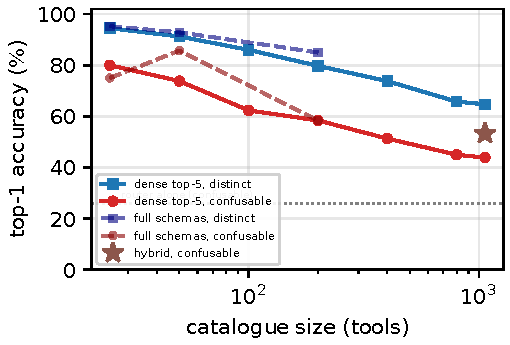
\includegraphics[width=0.95\columnwidth]{../figs/main_fig.pdf}
\caption{Top-1 selection accuracy versus catalogue size, split by
confusability. The confusable curve sits far below the distinct one at every
size, and full-schema prompting (dashed) does not close the gap. Dotted line:
the description-free router's confusable accuracy, flat in $N$ by
construction.}
\label{fig:retr}
\end{figure}

\subsection{Confusability moves the failure, it does not create it}
The cross-sectional gap is partly compositional: confusable queries belong to
large sibling families, over-represented at large $N$. For each of the 212
queries whose gold tool has confusers we therefore built two catalogues of the
\emph{same} size $N=200$ for the \emph{same} query: one excluding every
confuser, one with up to four forced in, displacing an equal number of random
distractors. Injecting confusers costs dense retrieval $-11.3 \pm 4.3$ points
of top-1 recall but only $-2.8 \pm 2.2$ of top-5 (95\,\% CIs over paired
differences); for BM25, $-2.8 \pm 2.6$ and $-1.9 \pm 1.8$.

This is a more useful result than a flat claim that retrieval breaks. Confusers
reliably displace the gold tool from rank~1, but rarely out of the top~5. In a
retrieve-then-select pipeline the gold tool therefore usually survives into the
candidate set, and the burden of telling \texttt{listServiceCatalog} from
\texttt{listResourceCatalog} is handed to whichever model does the final
selection. The question is whether that model can carry it.
